\chapter{الگوریتم های هوش مصنوعی مورد بررسی}
\section{شبکه های عصبی مصنوعی}
برای نوشتن مراجع پایان نامه، برای راحتی کار به صورت زیر عمل می‌کنیم:
\textbf{تست}
\section*{تستت}
\section{ماشین بردار پشتیبان}
در ابتدا مراجع را باید از سایت‌های معتبر بارگیری کنیم، مثلا برای ارجاع دادن به مقاله‌ی
\lr{A classification of some Finsler connections and their applications}
ابتدا به سایت
\href{scholar.google.com}{گوگل اسکولار} 
رفته و این مقاله را جستجو می‌کنیم. پس از پیدا کردن این مقاله، مانند شکل زیر، در زیر نام و چکیده‌ی مقاله، $5$ گزینه وجود دارد که عبارتند از:\\

\begin{enumerate}
\item \lr{ Cited by}

\item \lr{ Related articles}

\item \lr{ All 6 versions}

\item \lr{ Cite}

\item \lr{ Save}
\end{enumerate}
\begin{figure}[!h]
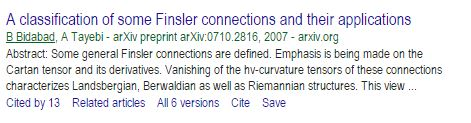
\includegraphics[height=3cm]{bidabad}
\caption{نمونه یک مقاله در گوگل اسکولار}
\end{figure}
در اینجا ما به گزینه‌ی چهارم یعنی
\lr{ Cite}
احتیاج داریم. بر روی آن کلیک کرده و پنجره‌ای مانند
\cref{fig.2}
باز می‌شود که دارای $4$ گزینه‌ی زیر است:
\begin{enumerate}
\item \lr{BibTeX}

\item \lr{EndNote}

\item \lr{RefMan}

\item \lr{RefWorks}
\end{enumerate}
\begin{figure}
\centering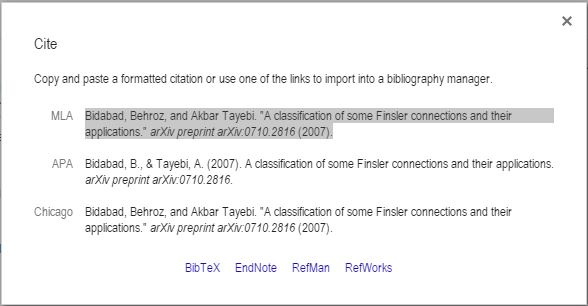
\includegraphics[scale=.6]{bibref}
\caption{پنجره‌ی باز شده در گوگل اسکولار}\label{fig.2}
\end{figure}
روی گزینه‌ی اول، یعنی
\verb;BibTeX;
کلیک کرده و همه‌ی نوشته‌های پنجره‌ی باز شده را مانند زیر، کپی کرده و در فایل
\verb;references.bib;
موجود در فایل
\verb;AUTthesis;
پیست می‌کنیم. سپس کلیدهای
\verb;Ctrl+s;
را می‌زنیم تا فایل ذخیره شود.\\
\begin{latin}
	\normalsize
\begin{verbatim}
@ article{bidabad2007classification,
title={A classification of some Finsler connections and their applications},
author={Bidabad, Behroz and Tayebi, Akbar},
journal={arXiv preprint arXiv:0710.2816},
year={2007}
}
\end{verbatim}
\end{latin}
\section{میانگین متحرک خودهمبسته یکپارچه}
برای ارجاع دادن به مقاله‌ی بالا، باید در جایی که می‌خواهید ارجاع دهید، دستور زیر را تایپ کنید:
\begin{latin}
\lr{$\backslash$cite\{bidabad2007classification\}}
\end{latin}
همانطور که مشاهده می‌کنید از کلمه‌ای که در سطر اول ادرس مقاله آمده (یعنی کلمه‌ی پس از
\lr{@article$\lbrace$})
استفاده کرده‌ایم. پس از دستور فوق، به صورت \cite{bidabad2007classification} و \cite{aa} مرجع خواهد خورد. توجه شود که در صورتی مراجع چاپ خواهند شد که در متن به انها ارجاع داده شده باشد. همچنین برای ارجاع چندتایی از دستور 
\lr{$\backslash$cite\{name1, name2,...\}}
استفاده کنید که به‌صورت \cite{najafi2008finsler, zakeri, najafi} ارجاع خواهند خورد.
\section{سری زمانی فازی}
ابتدا فایل
\verb;AUT_thesis.tex;
را باز کرده و آن را دو بار اجرا کنید. سپس حالت اجرا را از 
\verb;Build Quick;
به حالت
\verb;Bibtex;
تغییر داده و دوباره برنامه را اجرا کنید. دو بار دیگر برنامه را در حالت 
\verb;Build Quick;
اجرا کرده و نتیجه را مشاهده کنید. در این روش تمامی مراجع بر اساس اینکه کدام یک در متن زودتر به آن ارجع داده شده لیست خواهند شد.
\section{استدلال مبتنی بر مورد}
برای نوشتن مراجع فارسی باید به صورت دستی، در همان فایل قبلی به صورت زیر عمل می‌کنیم:
\begin{LTR}
\noindent\verb;@article{manifold,;\\
\verb;title={;منیفلد هندسه\verb;},;\\
\verb;author={;بیدآباد دکتربهروز \verb;},;\\
\verb;journal{; امیرکبیر صنعتی دانشگاه\verb;},;\\
\verb;year={1389},;\\
\verb;LANGUAGE={Persian};\\
\verb;};
\end{LTR}
همانطور که مشاهده می‌کنید تنها تفاوت آن با حالت مراجع انگلیسی، سطر آخر آن می‌باشد که زبان را مشخص می‌کند که حتماً باید نوشته شود.
\section{خلاصه}

به دلیل پیچیدگی واژه‌نامه‌های موجود در سایت پارسی لاتک، از روش زیر برای نوشتن واژه‌نامه استفاده کنید:

ابتدا با استفاده از اکسل، واژه های خود را یک‌بار براساس حروف الفبای فرسی و بار دیگر انگلیسی مرتب کنید. سپس واژه ها را در فایل \lr{dicen2fa} و \lr{dicfa2en} قرار دهید.

% \section{ساخت نمایه}\label{Namaye}
% \subsection{ساخت نمایه}
%  \begin{enumerate}

% \item
% کلمات مورد نظر خود مثلا \lr{word} با دستور \verb|\index{word}| ایندکس کنید.
% \item
% نحوه‌ی اجرای \lr{Make Index}   در ویرایشگرهای \lr{TeX Maker} و \lr{TeX Works}:
% \begin{itemize}
% \item  تک‌میکر: از منوی \lr{Tools} گزینه‌ی \lr{Xindy Make Index} را کلیک کنید یا از دکمه‌‌های میانبر \lr{Ctrl+Alt+I} استفاده کنید.

% \item  تک‌ورکز: ابتدا باید مثل عکس زیر تنظیم  و سپس گزینه‌ی \lr{Xindy Make Index}  انتخاب و روی دکمه‌ی سبز رنگ کلیک کنید یا از دکمه‌های  \lr{Ctrl+T} استفاده کنید.

% \begin{figure}[!h]
% \centerline{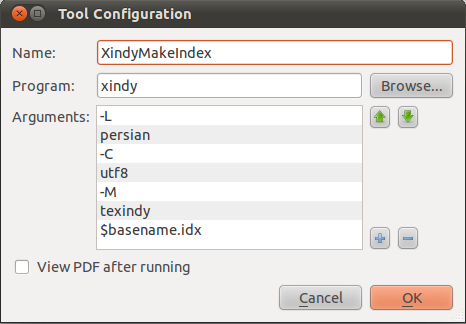
\includegraphics[width=.5\textwidth]{Xindy_Make_Index.png}}
% \caption{تنظیمات مربوط به تک‌ورکز}
% \end{figure}

% \end{itemize}
%  \end{enumerate}
 
 \index{کتاب}
\index{پارسی‌لاتک}
\index{بی‌دی}
\index{سوال}
\index{عنصر}
\index{گزینه}
\index{ژاکت}
\index{مرکز دانلود}
\index{اجرا}
\index{تک‌لایو}
\index{ثالث}
\index{جهان}
\index{چهار}
\index{حمایت}
\index{خواهش}
\index{دنیا}
\index{زی‌پرشین}
\index{ریحان}
\index{شیرین}
\index{صمیمی}
\index{ضمیر}
\index{طبیب}